\appendix

\section{Components of Dialog Interfaces}
\label{apx:int-photos}
In this section, we provide short descriptions and screenshots of every component of the user and assistant dialog interfaces.

\subsection{User's Interface}

Figure~\ref{fig:entity-quiz} shows the interface that we use to sample the user's prior knowledge of entities related to the topic.
To derive a diverse sample, we use Wikipedia page views as a proxy for how well known the entity is.
All experiments use the English Wikipedia dump generated on July 23, 2019.
We divide entity mentions into ten buckets based on the frequency of page views, and round-robin sample fifteen entities from those buckets.
The interface is shown before the user starts chatting with the assistant.
\begin{figure}[ht]
    \centering
    \nicebox{
        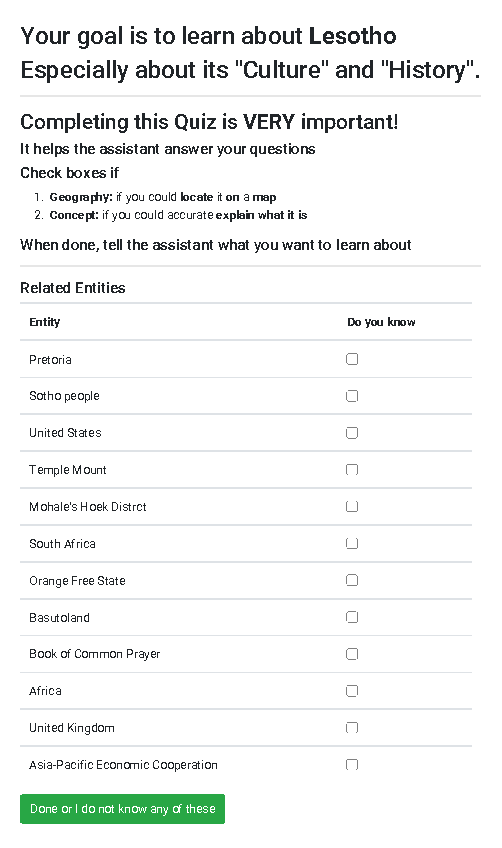
\includegraphics[width=\linewidth]{2020_emnlp_curiosity/figures/entity-quiz.pdf}
    }
    \caption{
        In this example, the user is assigned to learn about \topic{Lesotho}, specifically its \aspect{culture} and \aspect{history}.
        In addition to their training with guidelines and videos, we repeat the instructions here.
        The related entities span relatively common ones like the \entity{United States} or \entity{Africa} to less known ones such as \entity{Basutoland}.
    }
    \label{fig:entity-quiz}
\end{figure}

We elicit how ``interesting'' a user finds each of the assistant's messages through the like button in Figure~\ref{fig:like-button}.
Only users can ``like'' a message; the assistant cannot ``like'' user messages.
Users are instructed to ``like'' messages if they are ``interesting, informative and/or entertaining'' and ``relevant to their topic and/or aspects.''
They are specifically instructed not to ``like'' messages that are devoid of factual content, only express feelings, or only contain greetings or farewells.
\begin{figure*}[ht]
    \centering
    \nicebox{
        \begin{minipage}{.35\textwidth}
            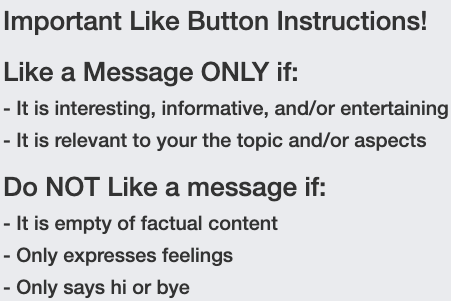
\includegraphics[width=\linewidth]{2020_emnlp_curiosity/figures/like-instructions}
        \end{minipage}
        \begin{minipage}{.60\textwidth}
            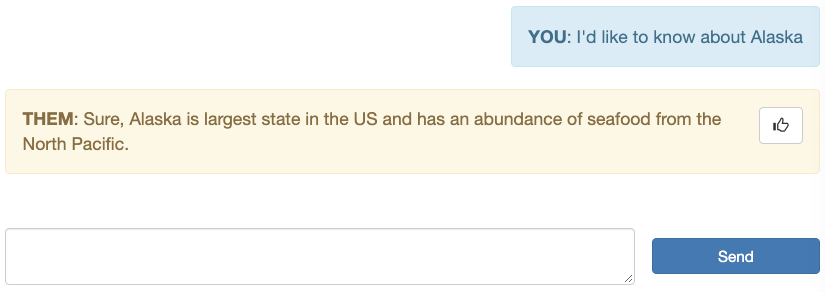
\includegraphics[width=\linewidth]{2020_emnlp_curiosity/figures/like-button}
        \end{minipage}
    }
    \caption{
        The user expresses the ``interestingness'' of the assistant's messages through a ``like'' button (right of message).
        The instructions are shown prominently in the full interface and repeated in training material.
    }
    \label{fig:like-button}
\end{figure*}

\paragraph{Switching Aspect}
Users are randomly assigned two aspects for each dialog and told to spend time discussing each.
The guidelines instruct them to spend at least two turns per topic, but we do not specify any further time requirements.
When the user changes aspects, we instruct them to click a button (Figure~\ref{fig:switch-aspect}) to indicate when and which aspect they are switching to.
Additionally, this event triggers a reset in the context we use to rank the assistant's facts.

\begin{figure}[ht]
    \centering
    \nicebox{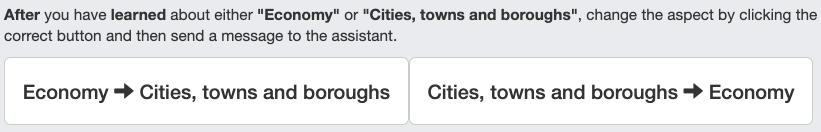
\includegraphics[width=.98\linewidth]{2020_emnlp_curiosity/figures/switch-aspect}}
    \caption{
        The user is assigned two aspects about their topic.
        After they are satisfied with what they have learned about the first aspect, they click a button and switch to the next aspect.
        While the button click is not communicated to the assistant (the user must send a corresponding message), it resets the fact contextualizer; we observe that without this, too many facts were related to the previous aspect.
    }
    \label{fig:switch-aspect}
\end{figure}

\subsection{Assistant Interface}

By design, we intend for most workers to not be familiar in depth with most of the geographic topics.
Thus, the most important responsibility of the assistant interface is to provide enough information---without overwhelming them---to be engaging conversational partners.
The first interface shown is a short description of the topic from either Simple Wikipedia or the English Wikipedia.
This component helps the assistant reach a general understanding of the topic so that they can choose better facts.
\begin{figure}[ht]
    \centering
    \nicebox{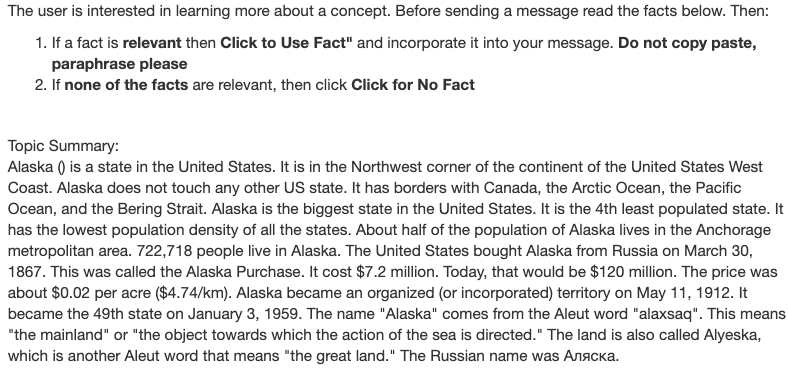
\includegraphics[width=.98\linewidth]{2020_emnlp_curiosity/figures/summary}}
    \caption{
        A short topic description is always visible to the assistant.
        The goal is to ensure the assistant always has a general understanding of the dialog topic.
    }
    \label{fig:summary}
\end{figure}

The most important component of the assistant interface is their list of available facts.
These facts have high textual similarity with the most recent three turns and are broken into three categories: facts related to entities the user knows about (rooted facts), facts related to an aspect (aspect facts), and facts from anywhere on the page (general facts).
Feedback from pilot collections showed that six facts was too few which caused a lack of relevant facts, but twelve facts overwhelmed annotators.
Thus, we use nine facts so that we can also balance equally across each type of fact.
When composing their reply, the assistant can use any number of facts as in Figure~\ref{fig:grounded-msg}.
To discourage verbatim copying, we disable the paste feature in javascript.
We also drop repeatedly unused facts.

\begin{figure*}[ht]
    \centering
    \begin{minipage}{\textwidth}
        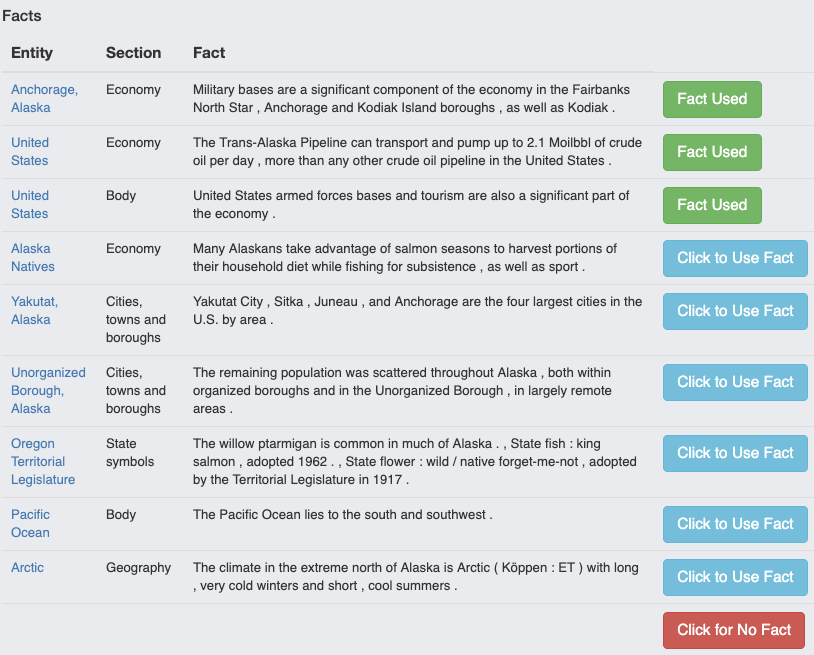
\includegraphics[width=\linewidth]{2020_emnlp_curiosity/figures/fact-bank}
    \end{minipage}
    \begin{minipage}{\textwidth}
        \nicebox{
            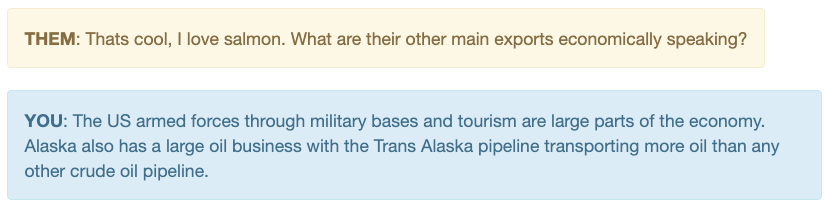
\includegraphics[width=.98\linewidth]{2020_emnlp_curiosity/figures/grounded-message}
        }
    \end{minipage}

    \caption{
        The assistant could incorporate any number of facts into their reply to the user.
        Their goal was to answer the user's immediate questions, and anticipate what information they would be most interested in.
    }
    \label{fig:grounded-msg}
\end{figure*}

\section{Dialog Act Annotation}
\label{apx:acts}
To annotate dialog acts, we create a separate annotation interface (Figure~\ref{fig:da-iface}).
The interface shows one dialog at a time, and the same annotator annotates all the utterances.
In addition to the utterances, the interface shows the topic, aspects, and sender of each message.
Lastly, we incorporate a ``Report Dialog'' feature to help identify and remove inappropriate dialogs.

\begin{figure*}[ht]
    \centering
    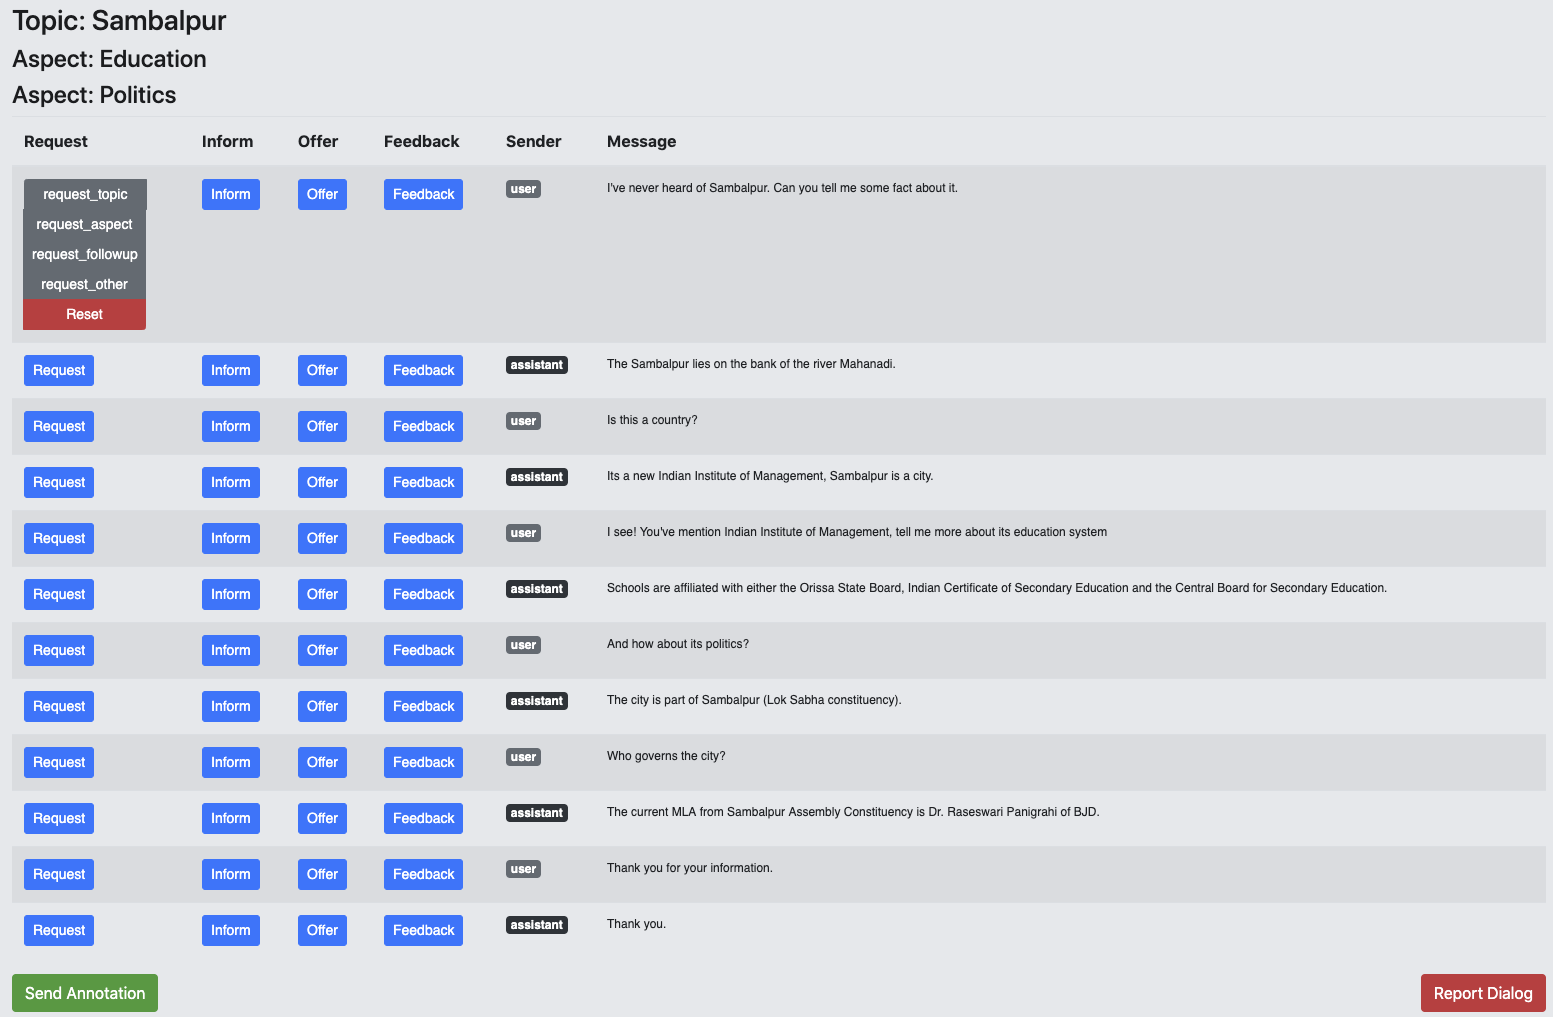
\includegraphics[width=\linewidth]{2020_emnlp_curiosity/figures/da-interface}
    \caption{
        To annotate dialog acts, we develop an interface that showed each utterance on a separate line.
        Annotators assign zero or more dialog acts to each utterance using grouped dropdowns.
    }
    \label{fig:da-iface}
\end{figure*}


\section{Sample Dialogs}
\label{apx:samples}
Tables~\ref{tab:dialog_example1} and~\ref{tab:dialog_example2} show \rover{} dialogs and highlight the dataset's features.
Typos and grammatical errors made by annotators are left unaltered.

\begin{table*}[t]
    \small
    \begin{center}
        \setlength\tabcolsep{3.5pt}
        \begin{tabular}{p{0.2cm}p{3.8cm}p{11cm}}
            \toprule[\heavyrulewidth]
              & \multicolumn{1}{r}{\textbf{Topic}:}          & \underline{Djibouti}                                                                                                                                                                                                                                                                                      \\
              & \multicolumn{1}{r}{\textbf{Aspects}:}        & \textit{Economy}, \textit{Politics}                                                                                                                                                                                                                                                                       \\
              & \multicolumn{1}{r}{\textbf{Known Entities}:} & France, Africa                                                                                                                                                                                                                                                                                            \\
            \midrule
              & Dialog Acts                                  & Messages                                                                                                                                                                                                                                                                                                  \\
            \midrule
            U & \texttt{request topic}                       & Hi can you tell me about Djibouti?                                                                                                                                                                                                                                                                        \\
            A & \texttt{inform response}                     & The country of Djibouti is officially called the Republic of Djibouti is located in the horn of Africa. It was created out of French Somaliland. It is also recorded the country was colonized by France in1800s and later gained its independence on June 27, 1977.                                      \\
            U & \texttt{request aspect}                      & Can you tell me about their Politics                                                                                                                                                                                                                                                                      \\
            A & \texttt{inform response}                     & After its independence, The country had two regiments commanded by the French officers. The country also maintains its close ties with Somalia, Ethiopia, France and the United States.                                                                                                                   \\
            U & \texttt{request aspect}                      & Any other information about the French and their impact of the politics?                                                                                                                                                                                                                                  \\
            A & \texttt{inform response}                     & There are no direct information on its effect on the country's politics but even though the country is already independent. The 13th Demi-brigade of the French Foreign Legion is still stationed in this country. It is also the largest french military presence abroad. commanded by a 3-star general. \\
            U & \texttt{request aspect}                      & Heavy French infeleunce. what other interesting inofrmation on politics do you have?                                                                                                                                                                                                                      \\
            A & \texttt{inform response}                     & In recent years, the country has improved its training techniques, military command, and information structure. They also became more self-reliant in supplying their military and assist in peacekeeping missions and provide military assistance to countries that officially ask them for help.        \\
            U & \texttt{request aspect, feedback positive}   & Wow Interesting, Can you now tell me about the economy they have?                                                                                                                                                                                                                                         \\
            A & \texttt{offer aspect}                        & Sorry, I do not have that information. But I can tell you more about Politics.                                                                                                                                                                                                                            \\
            U & \texttt{offer accept}                        & Sure                                                                                                                                                                                                                                                                                                      \\
            A & \texttt{inform response}                     & Camp Lemonnier is rented by the United State as a Naval Expeditionary Based for \$63 Million a year. While Japan and France each pays \$30 million a year and China pays \$20 Million a year.                                                                                                             \\
            U & \texttt{request other}                       & Lastly, any any fun facts?                                                                                                                                                                                                                                                                                \\
            A & \texttt{inform response}                     & I am not sure if this is a fun fact, but the country's gross domestic product expanded by more than 6\%. From \$341 Million to 1.5 Billion                                                                                                                                                                \\
            U & \texttt{}                                    & That's a huge increase. thank you for all your help                                                                                                                                                                                                                                                       \\
            A & \texttt{}                                    & You are welcome                                                                                                                                                                                                                                                                                           \\
            \bottomrule[\heavyrulewidth]
        \end{tabular}
    \end{center}
    \caption{Example dialog \#1 from \rover{}. (U: User, A: Assistant)}
    \label{tab:dialog_example1}
\end{table*}

\begin{table*}[t]
    \small
    \begin{center}
        \setlength\tabcolsep{3.5pt}
        \begin{tabular}{p{0.2cm}p{3.8cm}p{11cm}}
            \toprule[\heavyrulewidth]
              & \multicolumn{1}{r}{\textbf{Topic}:}          & \underline{British Columbia}                                                                                                                                                                         \\
              & \multicolumn{1}{r}{\textbf{Aspects}:}        & \textit{Government and politics}, \textit{Culture}                                                                                                                                                   \\
              & \multicolumn{1}{r}{\textbf{Known Entities}:} & Canada, Seattle                                                                                                                                                                                      \\
            \midrule
              & Dialog Acts                                  & Messages                                                                                                                                                                                             \\
            \midrule
            U & \texttt{request topic}                       & Hi! Can you help me learn some basic information about British Columbia? I don't know much except that it's located in Canada.                                                                       \\
            A & \texttt{inform response}                     & Yes, British Columbia is the westernmost province of Canada and is located between the Rocky Mountains and the Pacific Ocean.                                                                        \\
            U & \texttt{request aspect, feedback positive}   & I didn't know it was on the coast! What can you tell me about government and politics there?                                                                                                         \\
            A & \texttt{inform response}                     & One interesting fact about the government is that the Green Part plays a larger role in this province than it does in other provinces of Canada.                                                     \\
            U & \texttt{request followup, feedback positive} & Interesting. What can else you tell me about the Green Party?                                                                                                                                        \\
            A & \texttt{inform response}                     & The New Democratic Party and the Green Party caucuses together control 44 seats. Which seems like a lot but the British Columbia Green Party only takes up 3 of those 44 seats.                      \\
            U & \texttt{request aspect}                      & That's a pretty small influence. Can you tell me some fun culture facts about British Columbia?                                                                                                      \\
            A & \texttt{}                                    & I am sorry I do not have any information on their culture right now.                                                                                                                                 \\
            U & \texttt{request topic}                       & That's okay. What other fun facts can you share?                                                                                                                                                     \\
            A & \texttt{inform response}                     & Interestingly, Queen Victoria chose British Columbia to distinguish what was the British sector of the Columbia District from the United States which became the Oregon Territory on August 8, 1848. \\
            U & \texttt{request aspect}                      & So that's why it has "British" specifically as part of it's name! Makes sense. Are there any sports or outdoor activities that are popular in British Columbia?                                      \\
            A & \texttt{inform response}                     & Horseback riding is enjoyed by many British Columbians.                                                                                                                                              \\
            U & \texttt{}                                    & Thanks for your help today. Now I know more than I did before.                                                                                                                                       \\
            A & \texttt{}                                    & No problem, it was a pleasure.                                                                                                                                                                       \\
            \bottomrule[\heavyrulewidth]
        \end{tabular}
    \end{center}
    \caption{
        Example dialog \#2 from \rover{}. (U: User, A: Assistant).
        After mentioning the Green Party, the user asks a specific followup question; we use these interactions to estimate implicit preference.
    }
    \label{tab:dialog_example2}
\end{table*}

\section{Paraphrase Analysis and Samples}
\label{apx:para}
In Section~\ref{sec:para-analysis}, we describe the results of a manual analysis on two hundred and fifty assistant paraphrases.
Annotations were completed by the authors and shown in Table~\ref{tab:para}.
We break messages into four categories: paraphrases, copies, errors, and unrelated.
Paraphrases include messages that incorporate the selected fact and possibly additional information.
Copies include verbatim copying, cherry-picked phrases, and trivial contextualizations like replacing an entity with a pronoun.
Table~\ref{tab:par-ex} shows ten randomly selected paraphrases from the two hundred and fifty manual annotations.

\begin{table*}
    \small
    \centering
    \IfFileExists{2020_emnlp_curiosity/commit_auto_fig/paraphrase-table.tex}{\begin{tabular}{l l r r}
    \toprule Category & Label & Count & Percent \\ \midrule  Copy & verbatim & 68 & $27.2\%$\\  Copy & cherry-pick & 6 & $2.40\%$\\  Copy & context & 30 & $12.0\%$\\  \midrule Copy & Total & 104 & $41.6\%$\\\midrule\\  Paraphrase & paraphrase-correct & 111 & $44.4\%$\\  Paraphrase & paraphrase-multiple & 17 & $6.80\%$\\  \midrule Paraphrase & Total & 128 & $51.2\%$\\\midrule\\  Error & paraphrase-error & 5 & $2.00\%$\\  Unrelated & unrelated & 13 & $5.20\%$\\  \bottomrule Total && 250 & $100\%$\\  \bottomrule\end{tabular}}{\begin{tabular}{l l r r}
    \toprule Category & Label & Count & Percent \\ \midrule  Copy & verbatim & 68 & $27.2\%$\\  Copy & cherry-pick & 6 & $2.40\%$\\  Copy & context & 30 & $12.0\%$\\  \midrule Copy & Total & 104 & $41.6\%$\\\midrule\\  Paraphrase & paraphrase-correct & 111 & $44.4\%$\\  Paraphrase & paraphrase-multiple & 17 & $6.80\%$\\  \midrule Paraphrase & Total & 128 & $51.2\%$\\\midrule\\  Error & paraphrase-error & 5 & $2.00\%$\\  Unrelated & unrelated & 13 & $5.20\%$\\  \bottomrule Total && 250 & $100\%$\\  \bottomrule\end{tabular}}
    \caption{
        We analyze the paraphrases annotators use through manual categorization.
        The ``Copy'' category includes cherry-picked verbatim phrases, verbatim copies, and contextualized copies (e.g., changing a named entity to ``it'').
        The majority of paraphrases are correct and only incorporate the provided fact, but a few weave in other information.
        $7.2\%$ of paraphrases are either unrelated to the selected facts or paraphrase the fact incorrectly.
        Overall, $51.2\%$ of messages have valid paraphrases.
    }
    \label{tab:para}
\end{table*}


\begin{table*}
    \small
    \centering
    \begin{tabular}{p{15cm}}
        \toprule
        \textbf{Label:} paraphrase-correct                                                                                                                                                                                                                                                                                                                                                                           \\
        \textbf{Message:} I do not have the information available but I can tell you 10 million tones were exported annually for, Cardiff dock in the years leading up to the First World War.                                                                                                                                                                                                                       \\
        \textbf{Fact:} In the years leading up to the First World War , more than 10 million tonnes of coal was exported annually from Cardiff Docks .                                                                                                                                                                                                                                                               \\
        \midrule
        \textbf{Label:} copy                                                                                                                                                                                                                                                                                                                                                                                         \\
        \textbf{Message:} Media and journalists in Namibia are represented by the Namibia chapter of the Media Institute of 'southern Africa and the Editors Forum of Namibia.                                                                                                                                                                                                                                       \\
        \textbf{Fact:} Media and journalists in Namibia are represented by the Namibian chapter of the Media Institute of Southern Africa and the Editors ' Forum of Namibia .                                                                                                                                                                                                                                       \\
        \midrule
        \textbf{Label:} paraphrase-multiple                                                                                                                                                                                                                                                                                                                                                                          \\
        \textbf{Message:} The film industry has a rich history in Indonesian culture and the Indonesian Film Festival has been held regularly since 1955.                                                                                                                                                                                                                                                            \\
        \textbf{Fact:} Indonesia has held annual film festivals and awards , including the Indonesian Film Festival ( Festival Film Indonesia ) that has been held intermittently since 1955 .                                                                                                                                                                                                                       \\
        \midrule
        \textbf{Label:} context                                                                                                                                                                                                                                                                                                                                                                                      \\
        \textbf{Message:} EU means European Union. GDP per capital ranges from 188\% of EU average in Bratislava to 54\% in eastern Slovakia                                                                                                                                                                                                                                                                         \\
        \textbf{Fact:} GDP per capita ranges from 188 \% of EU average in Bratislava to 54 \% in Eastern Slovakia .                                                                                                                                                                                                                                                                                                  \\
        \midrule
        \textbf{Label:} paraphrase-correct                                                                                                                                                                                                                                                                                                                                                                           \\
        \textbf{Message:} Sudan was considered the 17th growing economy in the world. Its faster development of the country from oil profits.                                                                                                                                                                                                                                                                        \\
        \textbf{Fact:} Sudan , officially the Republic of the Sudan , is a country in Northeast Africa .                                                                                                                                                                                                                                                                                                             \\
        \midrule
        \textbf{Label:} paraphrase-correct                                                                                                                                                                                                                                                                                                                                                                           \\
        \textbf{Message:} There is a mountain range called the Annamite Range that runs along eastern border to Vietnam and another range, named Luang Prabang Range, near the Thailand border.                                                                                                                                                                                                                      \\
        \textbf{Fact:} The Mekong River forms a large part of the western boundary with Thailand , where the mountains of the Annamite Range form most of the eastern border with Vietnam and the Luang Prabang Range the northwestern border with the Thai highlands .                                                                                                                                              \\
        \midrule
        \textbf{Label:} copy                                                                                                                                                                                                                                                                                                                                                                                         \\
        \textbf{Message:} In 1603, the kingdoms of England, Scotland and Ireland were united in a personal union when James VI, king of Scots, inherited the crowns of England and Ireland and moved his court from Edinburgh to London; each country nevertheless remained a separate political entity and retained its separate political, legal and religious institutions. Would you like to know anything else? \\
        \textbf{Fact:} In 1603 , the kingdoms of England , Scotland and Ireland were united in a personal union when James VI , King of Scots , inherited the crowns of England and Ireland and moved his court from Edinburgh to London ; each country nevertheless remained a separate political entity and retained its separate political , legal , and religious institutions .                                 \\
        \midrule
        \textbf{Label:} copy                                                                                                                                                                                                                                                                                                                                                                                         \\
        \textbf{Message:} The A31 connects to the A35 at Bere Regis , and passes east through Wimborne and Ferndown to Hampshire where it later becomes the M27                                                                                                                                                                                                                                                      \\
        \textbf{Fact:} The A31 connects to the A35 at Bere Regis , and passes east through Wimborne and Ferndown to Hampshire , where it later becomes the M27 .                                                                                                                                                                                                                                                     \\
        \midrule
        \textbf{Label:} context                                                                                                                                                                                                                                                                                                                                                                                      \\
        \textbf{Message:} I'm not sure of that. One fact I do have is that by 1857, Chicago was Illinois' largest city.                                                                                                                                                                                                                                                                                              \\
        \textbf{Fact:} By 1857 , Chicago was Illinois 's largest city .                                                                                                                                                                                                                                                                                                                                              \\
        \midrule
        \textbf{Label:} paraphrase-correct                                                                                                                                                                                                                                                                                                                                                                           \\
        \textbf{Message:} On March 2, 2008, Dmitry Medvedev was elected President of Russia and Vladimir Putin became Prime Minister.                                                                                                                                                                                                                                                                                \\
        \textbf{Fact:} On 2 March 2008 , Dmitry Medvedev was elected President of Russia while Putin became Prime Minister .                                                                                                                                                                                                                                                                                         \\
        \bottomrule
    \end{tabular}
    \caption{
        A random sample of ten manually labeled paraphrases from the assistant.
        The top row indicates the label we (the authors) annotated, the middle row the message, and the bottom row the original fact from Wikipedia.
        The original fact is shown as displayed to crowd-workers including punctuation tokenization.
    }
    \label{tab:par-ex}
\end{table*}

\section{Like Prediction Comparison}
\label{apx:like-compare}
Like prediction is the one task where \charm{} was not the best model.
To better understand the differences between the \charm{} and \bert{} model, we randomly sample thirty dialogs in the test set and find assistant messages where the model predictions disagree.
Of the 202 assistant messages in the thirty dialogs, the \bert{} like prediction is correct 174 times ($86.1\%$) and \charm{} 170 times ($84.2\%$).
The models disagree on eight predictions ($3.96\%$); \bert{} is correct on six of these and \charm{} on the other two.
Table~\ref{tab:like-compare} shows the messages, predictions, and labels.
Although we might guess at why the predictions differ (e.g., perhaps something in the Florida dialog confused \bert{}), without further analysis we cannot establish causality.

\begin{table*}[ht]
    \small
    \centering
    \begin{tabular}{l l p{12cm}}
        \toprule
        Liked & Correct Model & Message                                                                                                                                                                          \\
        \midrule
        No    & \bert{}       & You are welcome!                                                                                                                                                                 \\
        \midrule
        Yes   & \bert{}       & I'm sorry I don't have anymore information about the etymology of Tunisia, but what I can tell you is that Tunisia Sports City is a whole sports city being constructed in Tunis \\
        \midrule
        Yes   & \bert{}       & Yes Buddhism is a dominant influence in Lao culture. It has been great helping you.                                                                                              \\
        \midrule
        Yes   & \charm{}      & Florida is a state in the southeast United States. What would you like to know?                                                                                                  \\
        Yes   & \bert{}       & They have an average daily temperature of 70.7, it's the warmest state in the U. S.                                                                                              \\
        Yes   & \charm{}      & Yes, I can. Florida is nicknamed the ``Sunshine State'', but severe weather is a common occurrence.                                                                              \\
        \midrule
        Yes   & \bert{}       & Hello, Indonesia is part of the Malay Islands and is in Southeast Asia. Would you like to know more about the history?                                                           \\
        Yes   & \bert{}       & I do not have etymologic information, would you like to know more about the economy? I can tell you thank Indonesia develops military and commuter aircraft.                     \\
        \bottomrule
    \end{tabular}
    \caption{
        To compare like prediction between models, we randomly sample thirty dialogs and obtain predictions from \charm{} and \bert{}.
        The table only shows messages where the model predictions disagree and indicates which model was correct.
        Dialogs are delineated by horizontal lines.
        Unfortunately, from only these examples we cannot determine why the \charm{} model errors in most of these predictions.
    }
    \label{tab:like-compare}
\end{table*}

\section{Model Training, Implementation, and Computation}
\label{apx:method:train}

We implement all models with PyTorch~\citep{paszke2017automatic} and \allennlp{}~\citep{Gardner2018AllenNLPAD}.
The learning rates for models is set using the built-in learning rate finder in \allennlp{}.
Model losses were optimized with Adam~\citep{Kingma2014AdamAM}; the \bert{} model uses a learning rate of $.0001$ and \charm{} a learning rate of $.001$ with otherwise default parameters.
We train for a maximum of forty epochs and early stop based on the sum of validation losses.
The \charm{} model uses batch size $64$ and the \bert{} model batch size $4$.
Our best model (\charm{}), has $26,970,475$ parameters, takes two hours and eighteen minutes to train, and early stops on epoch fifteen.
In our models, text encoders for utterances and facts share parameters.

Models were developed on a single machine with eighty Intel $2.0$GHz \abr{cpu}s, $256$\abr{gb} \abr{ram}, and eight Tesla V100 graphics cards.
Each model was trained and evaluated on a single graphics cards with hyper-parameter sweeps parallelized across the eight cards.

\allennlp{} configuration files and software dependencies (including version) are included in our code at \href{https://github.com/facebookresearch/curiosity}{github.com/facebookresearch/curiosity}.

\section{MS Marco Conversational Sample Queries}
\label{apx:marco}

Conversational \abr{ms marco} is a search dataset that partially inspired this work.
Assistant messages should prompt followup queries like in Table~\ref{tab:marco}.

\begin{table*}[t]
    \small
    \begin{center}
        \begin{tabular}{l}
            \toprule
            Query                                                                             \\
            \midrule
            What is a physician's assistant?                                                  \\
            What are the educational requirements required to become a physician's assistant? \\
            What does the education to become a physician's assistant cost?                   \\
            What's the average starting salary of a physician's assistant in the UK?          \\
            What's the average starting salary of a physician's assistant in the US?          \\
            What school subjects are needed to become a registered nurse?                     \\
            What is the physician's assistant average salary vs a registered nurse?           \\
            What the difference between a physician's assistant and a nurse practitioner?     \\
            Do nurse practitioners or physician's assistant's make more?                      \\
            Is a physician's assistant above a nurse practitioner?                            \\
            What is the fastest way to become a nurse practioner?                             \\
            How much longer does it take to become a doctor after being a nurse practitioner? \\
            What are the main breeds of goat?                                                 \\
            Tell me about boer goats.                                                         \\
            What goat breed is good for meat?                                                 \\
            Are angora goats good for meat?                                                   \\
            Are boer goats good for meat?                                                     \\
            What are pygmy goats used for?                                                    \\
            What goat breed is the best for fiber production?                                 \\
            How long do Angora goats live?                                                    \\
            Can you milk Angora goats?                                                        \\
            How many Angora goats can you have per acre?                                      \\
            Are Angora goats profitable?                                                      \\
            \bottomrule
        \end{tabular}
    \end{center}
    \caption{
        An exemplar query chain from the conversational variant of \abr{ms marco}.
        An ideal assistant should answer these questions \emph{and} inspire these types of followup questions.
    }
    \label{tab:marco}
\end{table*}
